\chapter[PPS reconstruction]{Reconstructing the Primordial Power Spectrum}
\label{chp:rec}

\begin{figure}[tp]
    \tikzsetnextfilename{spline}
    \includegraphics[width=\textwidth]{chapters/pps_reconstruction/plots/spline.tikz}
  \caption{%
    Linear spline reconstruction. The primordial power spectrum is reconstructed using \(\Nknots\) interpolation points \({\{(k_i,\Pknotj{i}):i=1,2,\ldots {\Nknots}\}}\). The end knots are fixed in \(k\) but allowed to vary in \({\Pknot}\), whereas the internal knots can vary subject to the constraint that \({k_1<k_2<\cdots<k_{\Nknots}}\).  The function \(\mathcal{P}_\mathcal{R}(k)\) is constructed within the range \([k_1,k_{\Nknots}]\) by interpolating logarithmically between adjacent knots (i.e., linearly in \(\log\)-\(\log\) space). Outside this range the function is extrapolated logarithmically.  The function \(\mathcal{P}_\mathcal{R}(k;\{k_i,\Pknotj{i}\})\) thus has \(2\Nknots-2\) parameters.  }\label{fig:linear_spline_reconstruction}
\end{figure}

In Chapter~\ref{chp:kd} I showed that all pre-inflationary universes take the same generic form. In addition, I demonstrated that the pre-inflationary phase could have produced a signature in the primordial power spectrum of curvature perturbations (Sections~\ref{cos:sec:comoving_curvature_perturbation}--\ref{cos:sec:CMB_stats}). Given this, it is instructive to ask what our current state of knowledge is of this spectrum, and whether observations are consistent with this prediction.

In this chapter, I therefore aim to reconstruct the primordial power spectrum of curvature perturbations from a model-independent standpoint, using modern Bayesian techniques. It is worth remarking that this analysis was enabled by the creation of PolyChord, which is detailed in Chapter~\ref{chp:pc}.

\section{Strategy}
In this chapter we model the PPS \(\PR(k)\) using a nested family of models where \(\PR(k)\) is piecewise linear in the \(\ln (\mathcal{P})\)-\(\ln (k)\) plane between a number of knots, \(\Nknots\), that is allowed to vary. The question arises as to how many knots one should use, and we address this question using Bayesian model comparison.  A family of priors is chosen where both the horizontal and vertical positions of the knots are allowed to vary. We examine the ``Bayes factor'' or ``Bayesian evidence'' as a function of \(\Nknots\) to decide how many knots are statistically justified.  A similar analysis has been performed by~\cite{vazquez_knots} and~\cite{knottedsky1}.  In addition, we marginalize over all possible numbers of knots to obtain an averaged reconstruction weighted according to the Bayesian evidence.

The generic prescription is illustrated in Fig.~\ref{fig:linear_spline_reconstruction}. \(\Nknots\) knots \(\{(k_i,\Pknotj{i})\,\): \(i=1,\ldots,\Nknots\}\) are placed in the \((k,\PR)\) plane and the function \(\PR(k)\) is constructed by logarithmic interpolation (a linear interpolation in \(\log\)-\(\log\) space) between adjacent points.  Outside the horizontal range \([k_1,k_N]\) the function is extrapolated using the outermost interval.

Within this framework, base \(\Lambda\)CDM arises when \({\Nknots=2}\)---in other words, when there are two boundary knots and no internal knots, and the parameters \(\Pknotj{1}\) and \(\Pknotj{2}\) (in place of \(A_\mathrm{s}\) and \(n_\mathrm{s}\)) parameterize the simple power-law PPS\@. There are also, of course, the four standard cosmological parameters \((\Omega_{\mathrm{b}} h^2\), \(\Omega_{\mathrm{c}} h^2\), \(100\theta_{\mathrm{MC}}\), and \(\tau\)), as well the numerous foreground parameters associated with the \Planck\ high-\(\ell\) likelihood, all of which are unrelated to the PPS\@.  This simplest model can be extended iteratively by successively inserting an additional internal knot, thus requiring with each iteration two more variables to parameterize the new knot position.


\begin{table}[tp]
  \centering
  \begin{tabular}{ll}
  Parameter range &
  Prior type
  \\
  \toprule
  \(10^{-4}\,\mathrm{Mpc}^{-1} = k_1< k_2 < \cdots < k_{\Nknots} = 0.3\,\mathrm{Mpc}^{-1}\) &
  log uniform (sorted)
  \\
  \( 2 < \ln\left(10^{10}\Pknotj{1}\right), \ldots ,\ln\left(10^{10}\Pknotj{{\Nknots}}\right) < 4 \)  &
  log uniform
  \\
  \(2\le \Nknots \le 10 \) &
  integer uniform
  \\
  \midrule
  \(0.019< \Omega_\mathrm{b} h^2 <0.025\) &
  uniform
  \\
  \(0.095< \Omega_\mathrm{c} h^2 <0.145\) &
  uniform
  \\
  \(1.03< 100\theta_\mathrm{MC} <1.05\) &
  uniform
  \\
  \(0.01< \tau< 0.4\) &
  uniform
  \\
  \bottomrule
\end{tabular}

  \caption{%
    Prior for moveable knot positions.  The \(\PR\) positions are distributed in a log-uniform manner across a wide range.  The \(k\) positions are also log-uniformly distributed across the entire range needed by \CosmoMC{} and are sorted so that \({k_1<\cdots<k_{\Nknots}}\).  When we marginalize over the number of knots, \(\Nknots\), we assume a uniform prior between 2 and 10. }\label{tab:P_k_priors} 
\end{table}

We run models for a variety of numbers of internal knots, \(\Nint =\Nknots -2\), evaluating the evidence for \(\Nint\).  Under the assumption that the prior is justified, the most likely, or preferred, model is the one with the highest evidence.  Evidences are evaluated using the \PolyChord{} sampler \citep{polychordletter,polychordpaper} in \CAMB{} and \CosmoMC{}. The use of \PolyChord{} is essential, as the posteriors in this parameterization are often multi-modal. Also, the ordered log-uniform priors on the \(k_i\) are easy to implement within the \PolyChord\ framework. All runs were performed with \(1000\) live points, oversampling the semi-slow and fast parameters by a factor of \(5\) and \(100\), respectively.

\begin{figure}[tp]
  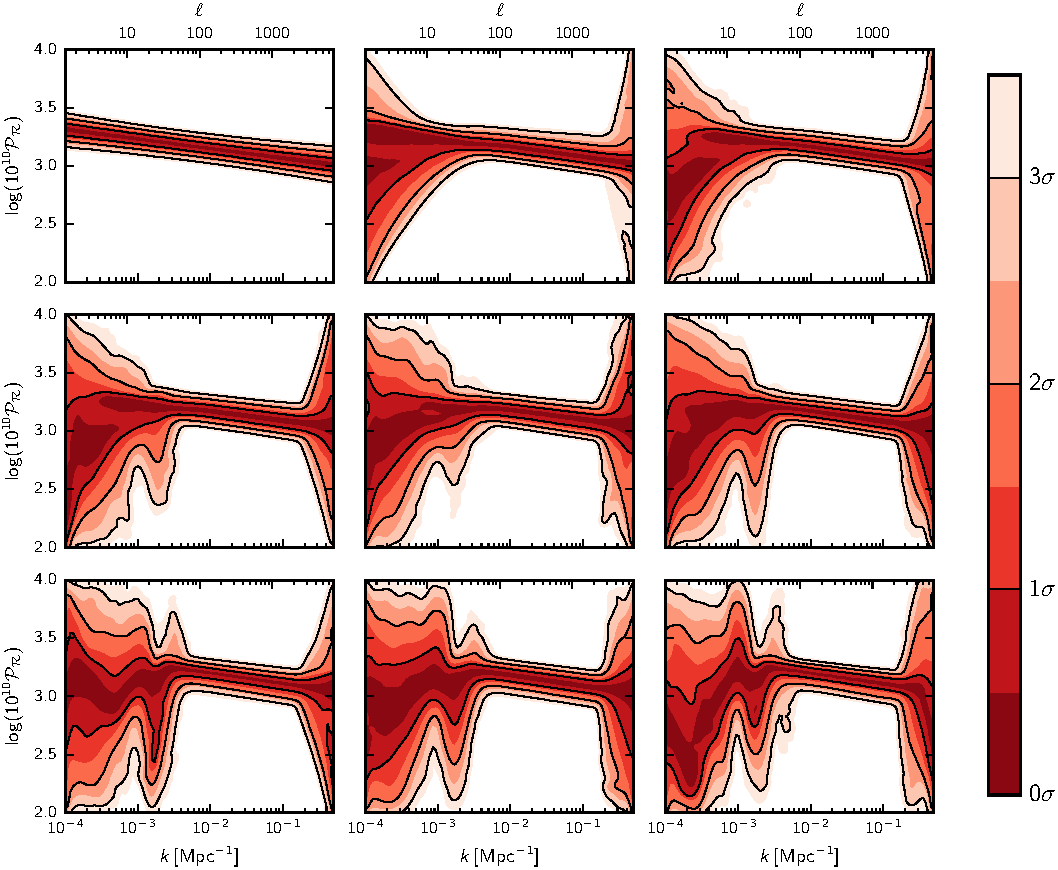
\includegraphics[width=\textwidth]{chapters/pps_reconstruction/figures/array}
  \caption{Bayesian movable knot reconstructions of the primordial power spectrum \(\PR(k)\) using \Planck\ TT data.  The plots indicate our knowledge of the PPS \(P(\PR(k)|k,N)\) for a given number of knots.  The number of internal knots \(\Nint\) increases (left to right and top to bottom) from \(0\) to \(8\).  For each \(k\)-slice, equal colours have equal probabilities. The colour scale is chosen so that darker regions correspond to lower-\(\sigma\) confidence intervals.  \(1\,\sigma \) and \(2\,\sigma \) confidence intervals are also sketched (black curves).  The upper horizontal axes give the approximate corresponding multipoles via \(\ell \approx k/D_\mathrm{rec}\), where \(D_\mathrm{rec}\) is the comoving distance to recombination.}\label{fig:Pkr0}
\end{figure}


\begin{figure}[tp]
  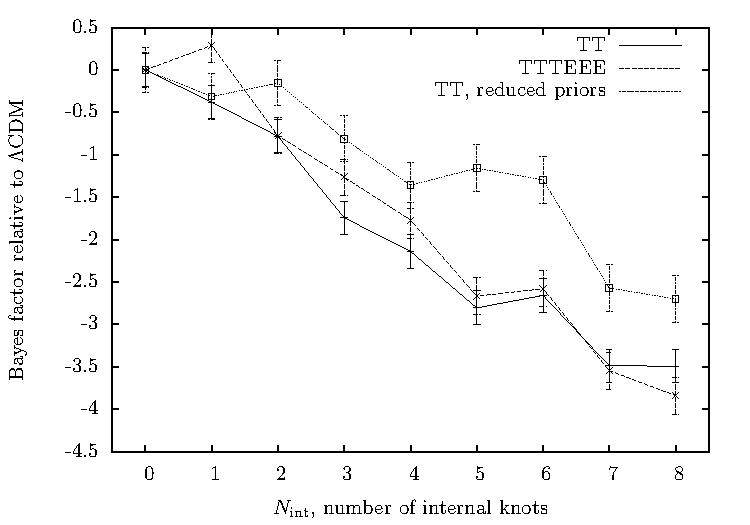
\includegraphics[width=\textwidth]{chapters/pps_reconstruction/figures/Bayes_PR}
  \caption{%
    Bayes factor (relative to the base \(\Lambda\)CDM model) as a function of the number of knots for three separate runs. Solid line: \Planck{} TT\@. Dashed line: \Planck{} TT,TE,EE\@. Dotted line: \Planck\ TT, with priors on the \(\Pknot\) parameters reduced in width by a factor of 2 (\(2.5<\ln(10^{10}\Pknot)<3.5\)).  }\label{fig:Bayes_Factors}
\end{figure}

\begin{figure}[tp]
  \begin{center}
    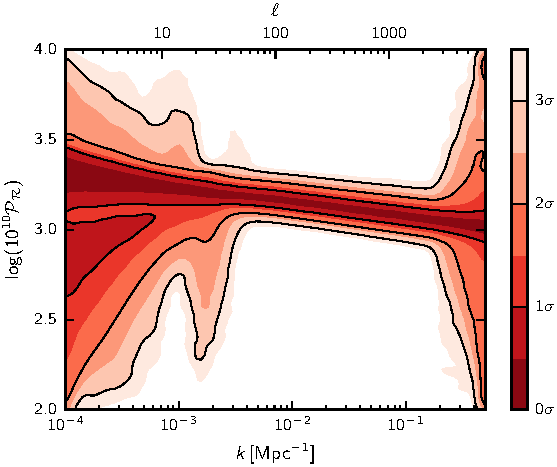
\includegraphics[width=\textwidth]{chapters/pps_reconstruction/figures/single}
  \end{center}
  \caption{%
    Bayesian reconstruction of the primordial power spectrum averaged over different values of \(N_\mathrm{int}\) (as shown in Fig.~\protect\ref{fig:Pkr0}), weighted according to the Bayesian evidence.  The region \({30<\ell<2300}\) is highly constrained, but the resolution is lacking to say anything precise about higher \(\ell\). At lower \(\ell\), cosmic variance reduces our knowledge of \(\PR(k)\).  The weights assigned to the lower \(\Nint\) models outweigh those of the higher models, so no oscillatory features are visible here.  }\label{fig:full_bayes_knots}
\end{figure}



Priors for the reconstruction and cosmological parameters are detailed in Table~\ref{tab:P_k_priors}.  We report evidence ratios with respect to the base \(\Lambda\)CDM case. The cosmological priors remain the same for all models, and this part of the prior has almost no impact on the evidence ratios.  The choice of prior on the reconstruction parameters \(\{\Pknotj{i}\}\) does affect the Bayes factor. \CosmoMC{}, however, puts an implicit prior on all models by excluding parameter choices that render the internal computational approximations in \CAMB{} invalid.  The baseline prior for the vertical position of the knots includes all of the range allowed by \CosmoMC{}, so slightly increasing this prior range will not affect the evidence ratios. If one were to reduce the prior widths significantly, the evidence ratios would be increased.  The allowed horizontal range includes all \(k\)-scales accessible to \Planck. Thus, altering this width would be unphysical.


After completion of an evidence calculation, \PolyChord\ generates a representative set of samples of the posterior for each model \(P(\Theta) \equiv P(\Theta|\mathrm{data},\Nint)\). We may use this to calculate a marginalized probability distribution for the PPS\@:
\begin{equation}
  P(\log\PR|k,\Nint) = \int \delta\left(\log\PR - \log\PR(k;\Theta)\right)P(\Theta)\:\d{\Theta}.
  \label{eqn:margPR}
\end{equation}
This expression encapsulates our knowledge of \(\PR\) at each value of \(k\) for a given number of knots.  Plots of this PPS posterior are shown in Fig.~\ref{fig:Pkr0} using \Planck\ TT data.


\section{Results}
If one considers the Bayesian evidences of each model, Fig.~\ref{fig:Bayes_Factors} shows that although no model is preferred over base \(\Lambda\)CDM, the case \(\Nint=1\) is competitive. This model is analogous to the broken-power-law spectrum of Sect.~4.4, although the models differ significantly in terms of the priors used. In this case, the additional freedom of one knot allows a reconstruction of the suppression of power at low \(\ell\). Adding polarization data does not alter the evidences significantly, although \(\Nint=1\) is strengthened. We also plot a \Planck\ TT run, but with the reduced vertical priors \({2.5<\ln\left(10^{10}\Pknot\right)<3.5}\).  As expected, this increases the evidence ratios, but does not alter the above conclusion.

For increasing numbers of internal knots, the Bayesian evidence monotonically decreases. Occam's razor dictates, therefore, that these models should not be preferred, due to their higher complexity. However, there is an intriguing stable oscillatory feature, at \(20\lesssim\ell\lesssim50\), that appears once there are enough knots to reconstruct it.  This is a qualitative feature predicted by several inflationary models (discussed in Sect.~9), and a possible hint of new physics, although its statistical significance is not compelling.

A full Bayesian analysis marginalizes over all models weighted according to the normalized evidence \(Z_{\Nint}\), so that:
\begin{equation}
  P(\log\PR|k) = \sum\limits_{\Nint} P(\log\PR|k,\Nint) Z_{\Nint},
  \label{eqn:margPR_full}
\end{equation}
as indicated in Fig.~\ref{fig:full_bayes_knots}.  This reconstruction is sensitive to how model complexity is penalized in the prior distribution. 


